\documentclass[12pt, a4paper]{article}

\usepackage[czech]{babel}
\usepackage[IL2]{fontenc}
\usepackage[utf8]{inputenc}
\usepackage{lmodern}  % lepší kvalita PDF

\usepackage[a4paper,top=3cm,bottom=3cm,left=3cm,right=3cm,marginparwidth=1.75cm]{geometry}

\usepackage{graphicx}
\usepackage{titling}
\usepackage{enumitem}
\usepackage{caption}
\usepackage{float}
\usepackage{pdfpages}

\usepackage{pkg-custom-commands}
\usepackage{pkg-url}

% údaje na titulní straně
\title{Implementace\\Data Encryption Standard}
\def \thesubtitle {Semestrální práce z předmětu KIV/BIT}
\author{Patrik Harag}
\def \theauthoremail {harag@students.zcu.cz}
\def \theauthorid {(A15B0034P)}

\begin{document}

\begin{titlepage}
	\begin{figure}
		
\includegraphics[height=50mm]{img-fav-logo}
	\end{figure}
	
	\centering
	{\large \hspace{1mm} \par} % tady musí být nějaký text jinak nefunguje vertikální odsazení
	\vspace{15ex}
	
	{\scshape\Large \thesubtitle \par}
	\vspace{1.5ex}
	{\huge\bfseries \thetitle \par}
	\vspace{2ex}
	{\Large\itshape \theauthor \par}
	\vspace{2ex}
	{\texttt{\theauthoremail} \par}
	\vspace{1ex}
	{\texttt{\theauthorid} \par}
	\vspace{5ex}
	{{Celková doba řešení: 24 h} \par}
	
	\vfill

	{\today\par}
\end{titlepage}

\section{Zadání}
Předmětem této práce je implementace blokové symetrické šifry \emph{Data Encryption Standard} (\emph{DES}) s vybranými operačními módy.

\section{Analýza}
\paragraph{Data Encryption Standard}
Je symetrická bloková šifra.
V USA byla od sedmdesátých let standardem pro šifrování dat v civilních státních organizacích, až do roku 2002, kdy byla nahrazena šifrou \emph{Advanced Encryption Standard}.
Archivovaná verze původního standardu \cite{fips46}, byla použita jako hlavní zdroj informací o DES.

Šifra pracuje s 64bitovým blokem dat a 16 klíči o 48 bitech.
Dešifrování se liší pouze opačným pořadím klíčů.
Vstupní blok je nejprve permutován podle tabulky definované v \cite{fips46} a je rozdělen na levou a pravou část.
Následuje 16 iterací:
\[ R_{n-1} = L_n \]
\[ L_{n-1} = R_n \mathbin{\oplus} f(L_n, K_n) \]
kde $L_n$ je levá strana iterace $n$, $P_n$ je pravá strana iterace $n$, $K_n$ je klíč iterace $n$, operátor $\mathbin{\oplus}$ je XOR a funkce $f$ je Feistelova funkce.
Po poslední iteraci jsou strany naposledy prohozeny a sjednoceny.
Vzniklý blok je permutován podle tabulky definované v \cite{fips46}.
Celé schéma je vidět na obr. \ref{fig:img-des}.
\begin{figure}
	\centering
	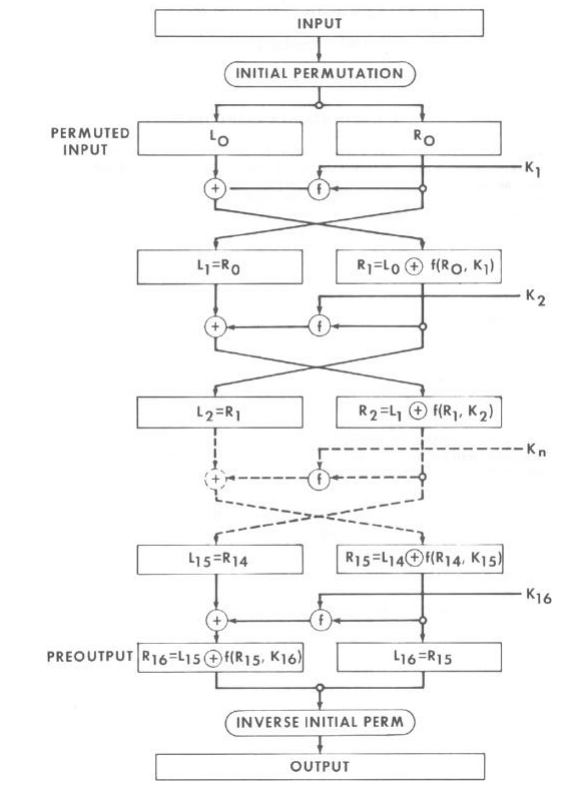
\includegraphics[width=1\linewidth]{img-des}
	\caption{Schéma algoritmu DES \cite{fips46}}
	\label{fig:img-des}
\end{figure}

Feistelova funkce se skládá z expanze vstupního půl-bloku na 48 bitů podle tabulky definované v \cite{fips46}, po kterém následuje XOR s klíčem.
Vzniklý mezivýsledek je rozdělen na 8 částí po 6 bitech.
Tyto části jsou podle tabulek z \cite{fips46} nahrazeny 4bitovými čísly (první + poslední bit = řádek, prostřední 4 bity = sloupec)  a opět sloučeny do půl-bloku.
Vzniklý půl-blok je permutován podle tabulky definované v~\cite{fips46}.
Celé schéma je vidět na obr. \ref{fig:img-feistel-function}.
\begin{figure}
	\centering
	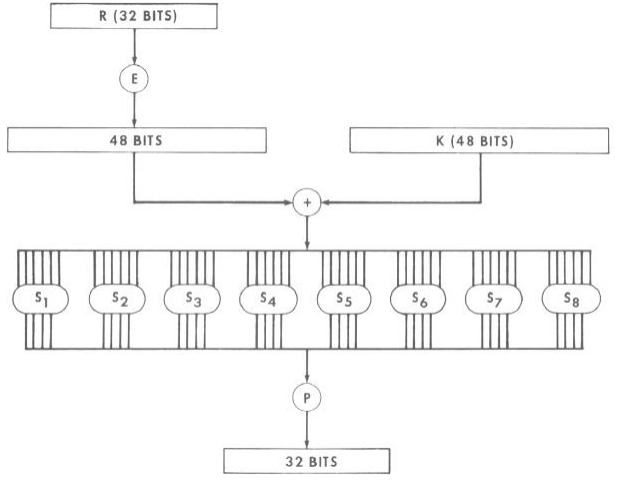
\includegraphics[width=0.8\linewidth]{img-feistel-function}
	\caption{Schéma Feistelovy funkce \cite{fips46}}
	\label{fig:img-feistel-function}
\end{figure}

Oněch 16 klíčů o 48 bitech, které se používají v jednotlivých iteracích algoritmu je možné vygenerovat z jednoho 64bitového klíče.
Schéma ukazuje obr. \ref{fig:img-keygen}.
\begin{figure}
	\centering
	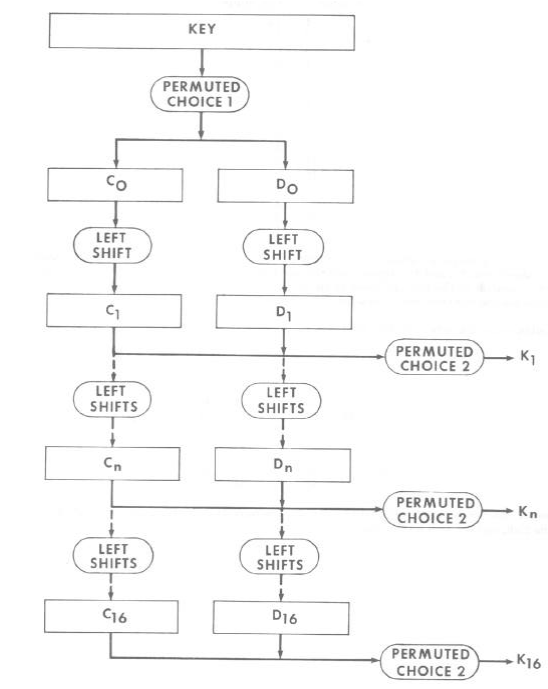
\includegraphics[width=0.6\linewidth]{img-keygen}
	\caption{Schéma generování klíčů \cite{fips46}}
	\label{fig:img-keygen}
\end{figure}

\paragraph{Operační módy}
DES pracuje pouze s 64bitovými bloky dat.
Existuje více způsobů, jak přistoupit k šifrování/dešifrování většího počtu boků.
Souhrnně se jim říká operační módy a nejedná se pouze o záležitost DES, ale blokových šifer obecně.

Nejjednodušší mód se nazývá \emph{Electronic Codebook} (ECB) a spočívá v pouhém rozdělení vstupních dat na bloky, které šifra zvládne a jejich postupném zašifrování/dešifrování.

Další významný mód se nazývá \emph{Cipher Block Chaining} (CBC) a řeší jeden z~problémů ECB, kterém je skutečnost, že stejné vstupní bloky jsou po zašifrování reprezentovány stejně.
Docílí toho tak, že při šifrování provádí XOR bloku s předešlým blokem po zašifrování a teprve tento výsledek zašifruje.
Při dešifrování naopak provádí XOR právě dešifrovaného bloku s předešlým blokem před dešifrováním.
Vyžaduje tzv. inicializační vektor pro první blok.

\paragraph{Možnosti paralelizace} 
Iterativní charakter DES paralelizaci dosti komplikuje, ale efektivní paralelizaci by mělo být možné snadno zavést na úrovni operačního módu ECB.

\section{Návrh}
Bude implementována šifra DES s módy \emph{Electronic Codebook} (ECB), paralelní ECB a \emph{Cipher Block Chaining} (CBC).
Dále bude vytvořen program s CLI, který umožní zašifrování a dešifrování souborů.
Jádro bude naprogramováno v jazyce Java, testy a nekritická logika v dynamickém jazyce Groovy.

\section{Popis implementace}
Byl vytvořen program umožňující šifrování a dešifrování pomocí DES.

\subsection{Seznam tříd}
\begin{itemize}
	\item \code{Main} -- Vstupní třída zpracovávající parametry příkazové řádky.
	\item \code{DES} -- Poskytuje metody pro šifrování a dešifrování vstupních proudů (třída \code{InputStream}) pomocí DES.
	\item \code{DESCore} -- Stará se o šifrování a dešifrování jednoho bloku.
	\item \code{DESKeyGenerator} -- Třída pro generování klíčů. Vygeneruje 16 klíčů o 48 bitech z jednoho 64 bitového klíče.
	\item \code{BitUtils} -- Pomocné metody pro práci s bloky.
	\item \code{LongInputStream} -- Vlastní implementace vstupního proudu pro načítání čísel typu \code{long} pracující s třídou \code{InputStream}.
	\item \code{LongInputStreamPlainText} -- Speciální typ \code{LongInputStream} pro plain text.
	\item \code{LongInputStreamCipherText} -- Speciální typ \code{LongInputStream} pro zašifrovaný text.
	\item \code{LongOutputStream} -- Vlastní implementace výstupního proudu pro zápis čísel typu \code{long} pracující s třídou \code{OutputStream}.
\end{itemize}

\subsection{Řešené problémy}
\paragraph{Zarovnání do bloku}
DES je navržen tak, že pracuje pouze s 64bitovými bloky.
Pokud nastane situace, kdy potřebujeme zašifrovat kratší blok, musíme ho prodloužit na 64 bitů.
Po dešifrování však nastane situace, kdy je dešifrovaný blok jiný než blok na vstupu a není možné jednoznačně určit, zda byl prodloužen.

Tento problém jsem vyřešil tak, že na začátek zašifrovaného souboru ukládám délku původního souboru.
Třídy \code{LongInputStream}, \code{LongInputStreamPlainText}, \code{LongInputStreamCipherText} a \code{LongOutputStream} vznikly pouze proto, aby řešily tento problém.

\section{Uživatelská dokumentace}

\subsection{Sestavení}
Pro sestavení je vyžadován JDK 8 a Gradle. Sestavení spustíme příkazem:

\code{gradle build}

\subsection{Spuštění}
Pro spuštění je vyžadován JRE 8. Program spustíme příkazem:

\code{java -jar \tag{program} \tag{parametry}}

\paragraph{Seznam parametrů}
\begin{itemize}
	\item \code{-in \tag{soubor}} \hspace{10pt} vstupní soubor,
	\item \code{-out \tag{soubor}} \hspace{10pt} výstupní soubor,
	\item \code{-e} nebo \code{-encrypt} \hspace{10pt} provede šifrování vstupního souboru -- výchozí,
	\item \code{-d} nebo \code{-decrypt} \hspace{10pt} provede dešifrování výstupního souboru,
	\item \code{-k \tag{číslo}} nebo \code{-key \tag{klíč}} \hspace{10pt} 64bitový klíč v hexadecimální soustavě,
	\item \code{-ecb} \hspace{10pt} použití módu Electronic Codebook (ECB) -- výchozí mód,
	\item \code{-pecb} nebo \code{-parallel-pecb} \hspace{10pt} použití módu paralelní ECB,
	\item \code{-cbc} \hspace{10pt} použití módu Cipher Block Chaining (CBC),
	\item \code{-iv \tag{číslo}} \hspace{10pt} inicializační vektor pro CBC v hexadecimální soustavě,
\end{itemize}
U přepínačů na velikosti písmen nezáleží.
Pokud se budu parametry opakovat, dojde k jejich přepsání.
Projekt obsahuje ukázkový dávkový soubor s názvem \code{example.bat}, který obsahuje několik příkazů pro inspiraci.

\section{Závěr}
Práce obsahuje implementaci šifry \emph{Data Encryption Standard} (\emph{DES}) s programem pro šifrování a~dešifrování souborů.

Implementace šifry je přímočará a bez optimalizací, které by zastíraly podstatu věci, je proto vhodná spíše pro vzdělávací účely než běžné použití.
Paralelizovaný mód ECB zašifruje/dešifruje soubor na čtyřjádrovém CPU Intel Core i5-4570 zhruba za 1/3 času oproti klasickému ECB (platí pro větší soubory).

Správnost je ověřena pomocí jednotkových testů s použitím knihovny JUnit 4.


\bibliographystyle{plain}
\bibliography{references}

\end{document}